\chapter{Architectural Views for Our Suggestions to Improve the Existing System} \label{suggest}

\section{Functional View}

\subsection{Stakeholders’ Uses of This View}

\begin{itemize}
  \item \textbf{Marine Ecologists}
    \begin{itemize}
      \item Use the \emph{Data Catalog Service} to search, filter and retrieve clips by location, date, or species metadata.
      \item Leverage the \emph{Visualization Toolkit} functions to generate spatial–temporal maps of species occurrences.
    \end{itemize}

  \item \textbf{Citizen Scientists}
    \begin{itemize}
      \item Rely on the \emph{Tutorial Manager} to access step-by-step guidance and contextual help before annotating.
      \item Submit annotations through \emph{Workflow 1} and \emph{Workflow 2} and receive quality feedback via the \emph{Quality Control Service}.
    \end{itemize}
  \newpage
  \item \textbf{ML Engineers \& Developers}
    \begin{itemize}
      \item Invoke the \emph{Hyperparameter Tuner} to automate model parameter sweeps and improvements.
      \item Register and retrieve model artifacts through the \emph{Model Registry} for versioning, rollback, and A/B testing.
      \item Call the \emph{Inference API} for batch or online predictions in downstream applications.
    \end{itemize}

  \item \textbf{System Administrators}
    \begin{itemize}
      \item Schedule and monitor the \emph{Backup Manager} to ensure hot/cold storage snapshots and disaster-recovery workflows.
      \item Configure and enforce access control via the \emph{Auth Service}.
      \item Dispatch alerts and system notifications using the \emph{Notification Service}.
    \end{itemize}

  \item \textbf{Sponsors \& Funders}
    \begin{itemize}
      \item Evaluate the \emph{Quality Control Service} and \emph{Backup Manager} as risk-mitigation mechanisms.
      \item Assess the \emph{Data Catalog} and \emph{Model Registry} for system extensibility, reproducibility, and governance.
    \end{itemize}
\end{itemize}

\subsection{Component Diagram}

\begin{figure}[H]
    \centering
    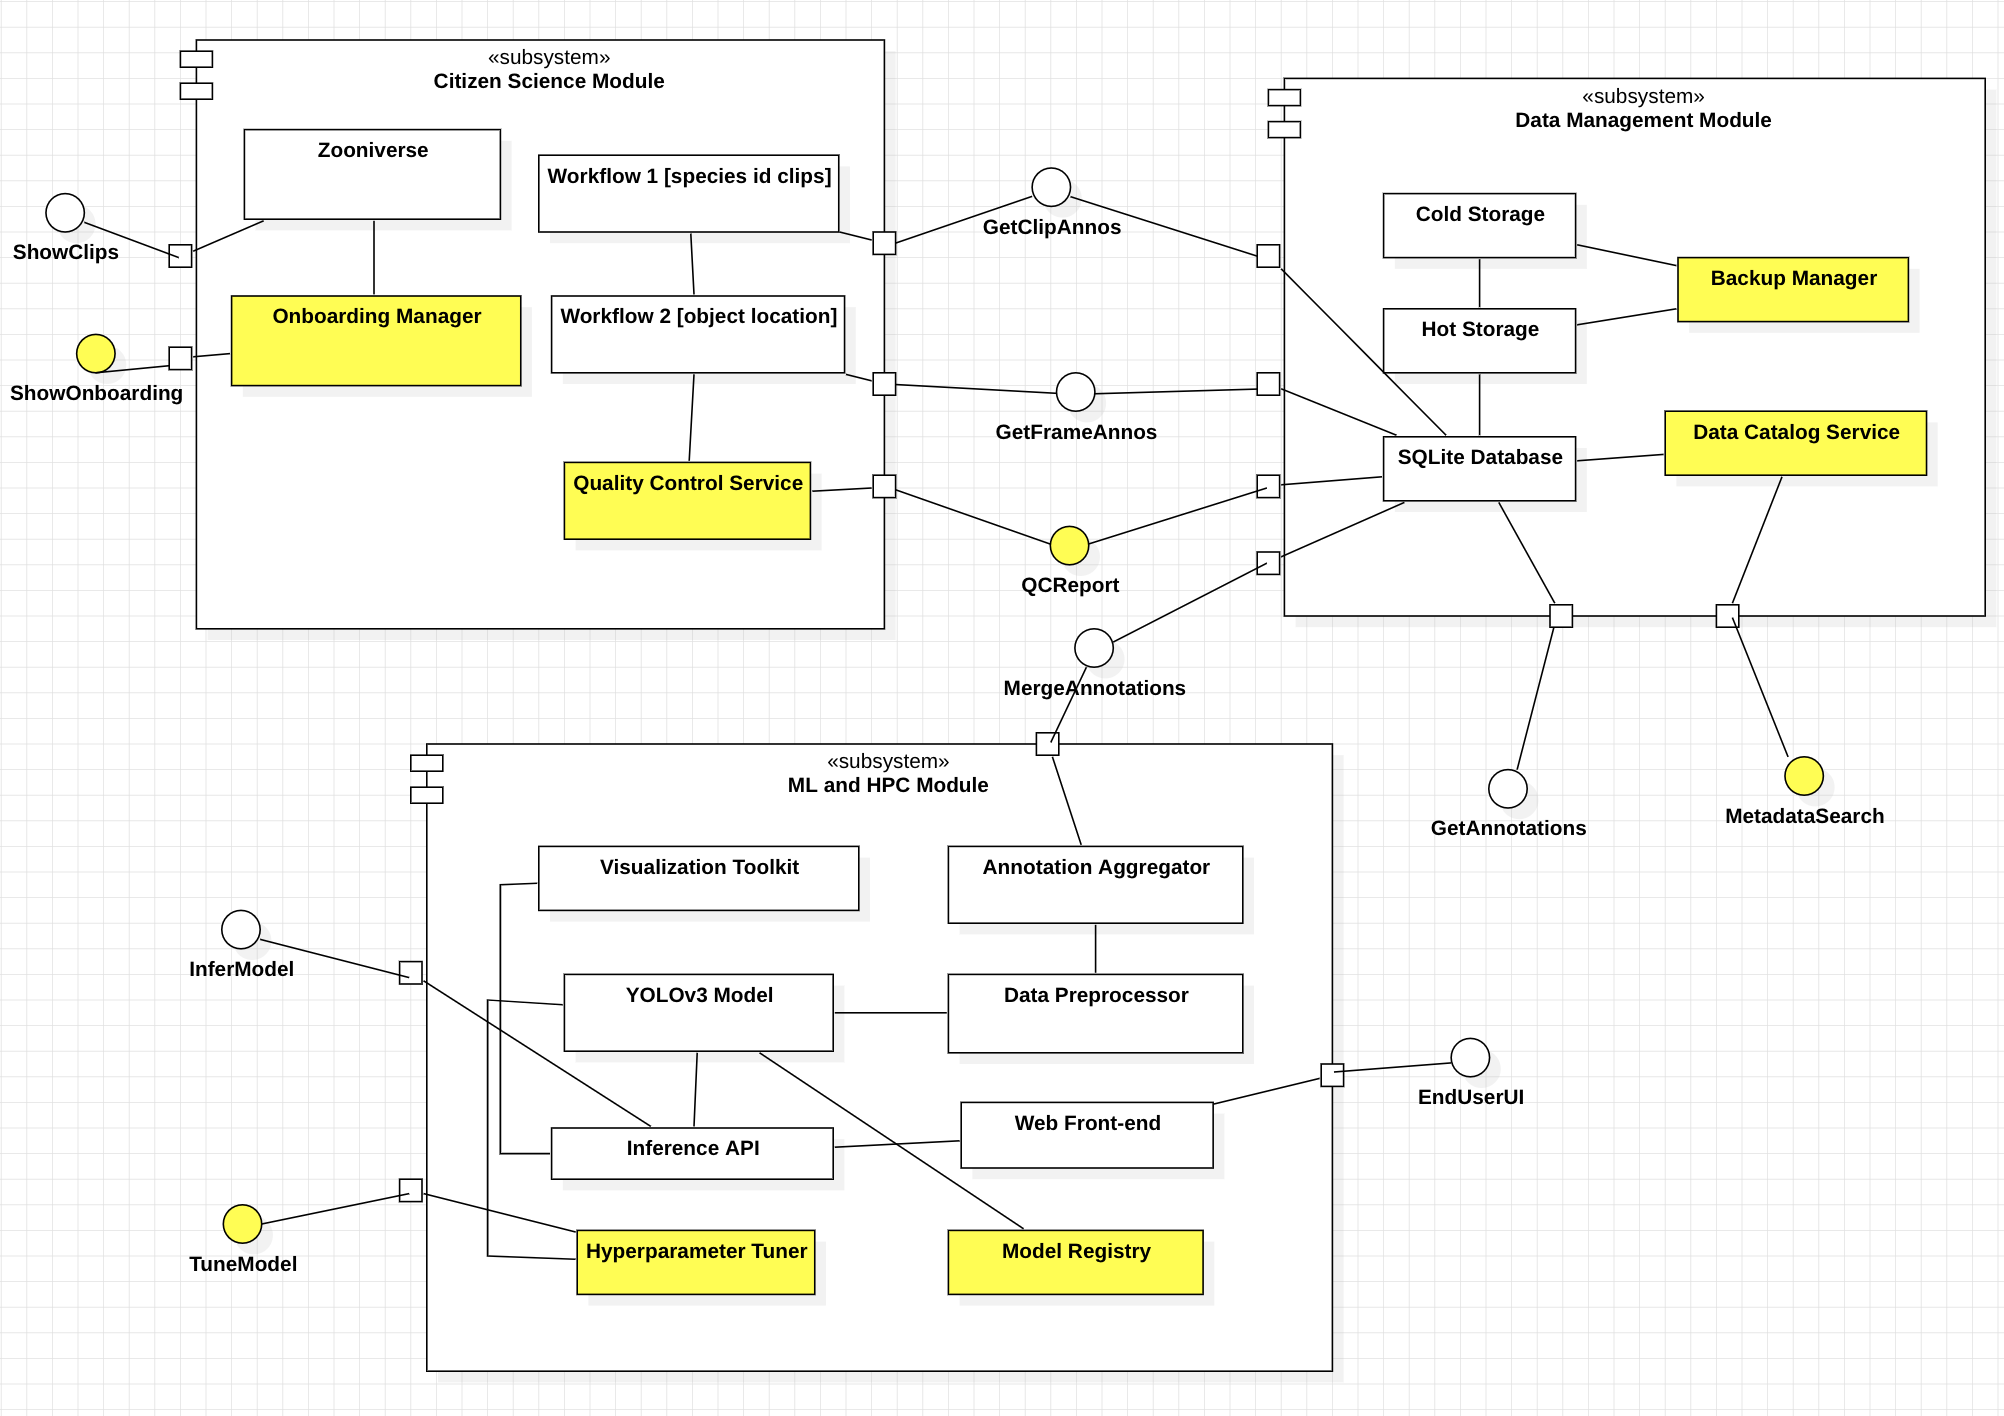
\includegraphics[width=1 \textwidth]{Figures/ImpComponentDiagram.png}
    \caption{Improved Component Diagram \label{Fig:Improved Component Diagram}}
\end{figure}

We made the following additions to our component diagram, as can be seen from Figure \ref{Fig:Improved Component Diagram}:

\paragraph{Data Management Module}
\begin{itemize}
  \item \textbf{Data Catalog Service} (\verb|<<component>>|)  
    \begin{itemize}
      \item Provides searchable index of clip/frame metadata  
      \item Interface: \verb|«MetadataSearch»|
    \end{itemize}
  \item \textbf{Backup Manager} (\verb|<<component>>|)  
    \begin{itemize}
      \item Automates snapshots and replication of hot/cold storage  
      \item Interface (internal): \verb|«Backup»|
    \end{itemize}
\end{itemize}

\paragraph{Citizen Science Module}
\begin{itemize}
  \item \textbf{Quality Control Service} (\verb|<<component>>|)  
    \begin{itemize}
      \item Applies consensus QC rules and flags low‐confidence annotations  
      \item Interface: \verb|«QCReport»|
    \end{itemize}
  \item \textbf{Tutorial Manager} (\verb|<<component>>|)  
    \begin{itemize}
      \item Hosts onboarding tutorials and context‐sensitive help  
      \item Interface: \verb|«ShowOnboarding»|
    \end{itemize}
\end{itemize}

\paragraph{Machine Learning \& HPC Module}
\begin{itemize}
  \item \textbf{Hyperparameter Tuner} (\verb|<<component>>|)  
    \begin{itemize}
      \item Automates parameter sweeps and optimization  
      \item Interface: \verb|«TuneModel»|
    \end{itemize}
  \item \textbf{Model Registry} (\verb|<<component>>|)  
    \begin{itemize}
      \item Version‐controls trained models and artifacts  
      \item Interface (internal): \verb|«ModelVersion»|
    \end{itemize}
\end{itemize}

These additions boost discoverability, reliability, quality control, and manageability across all modules.

\subsection{Internal Interfaces}

\begin{figure}[H]
    \centering
    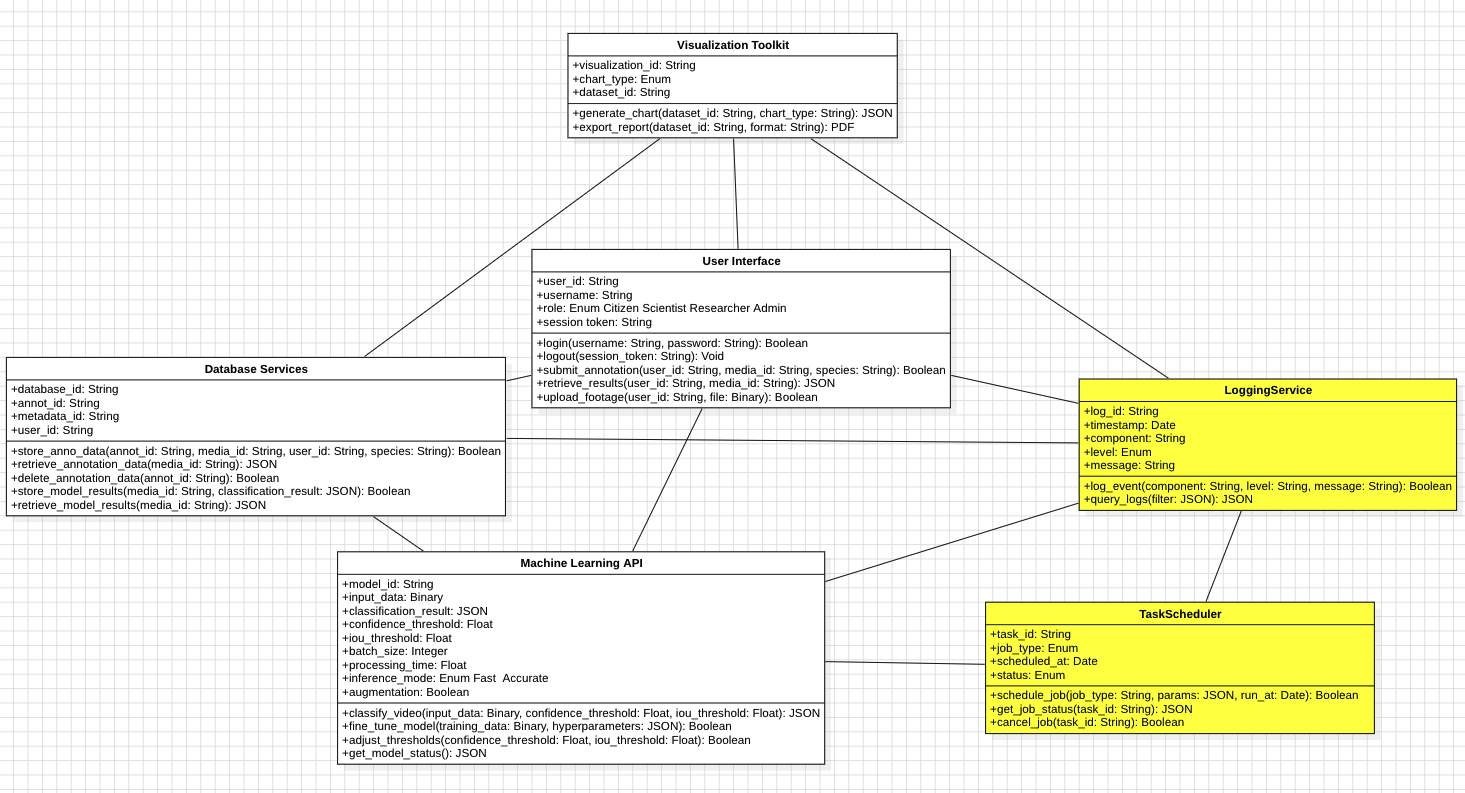
\includegraphics[width=1 \textwidth]{Figures/ImpInternalInterface.png}
    \caption{Improved Internal Interfaces Class Diagram \label{Fig:Improved Internal Interfaces Class Diagram}}
\end{figure}

As can be seen from the Figure \ref{Fig:Improved Internal Interfaces Class Diagram}, we added the following internal interfaces:
\paragraph{TaskScheduler Interface:}
This interface handles the queuing, scheduling and lifecycle management of all asynchronous, compute‐intensive jobs (e.g.\ video classification, model fine‐tuning, report export). KSO submits a JSON payload containing the \texttt{jobType}, parameters and desired start time and receives back a \texttt{taskId}; it can then poll that \texttt{taskId} via REST (or consume status events via a message queue) to observe transitions (“\texttt{PENDING}”, “\texttt{RUNNING}”, “\texttt{COMPLETED}”, “\texttt{FAILED}”), cancel pending work, or retrieve error details. Under the hood it persists tasks in a durable queue (e.g.\ RabbitMQ or a database table) to guarantee reliable delivery, survive restarts, and decouple heavy workloads from the core service.

\paragraph{LoggingService Interface:}
This interface collects, stores and serves all operational and audit logs emitted by KSO components (UI, Database Services, Machine Learning API, TaskScheduler, Visualization Toolkit). Each subsystem invokes a REST or gRPC call with a JSON record—containing \texttt{timestamp}, \texttt{component}, \texttt{level} and \texttt{message}—and receives a Boolean acknowledgment. Consumers (e.g.\ dashboards or alerting tools) can query the service with JSON‐encoded filters (time ranges, severity, component) to retrieve matching entries. The LoggingService backs onto an append‐only store with configurable retention and guarantees write latency $ \leq $ 2 ms and query latency $ \leq $ 200 ms for recent data.

\subsection{Interaction Patterns}
\begin{figure}[H]
    \centering
    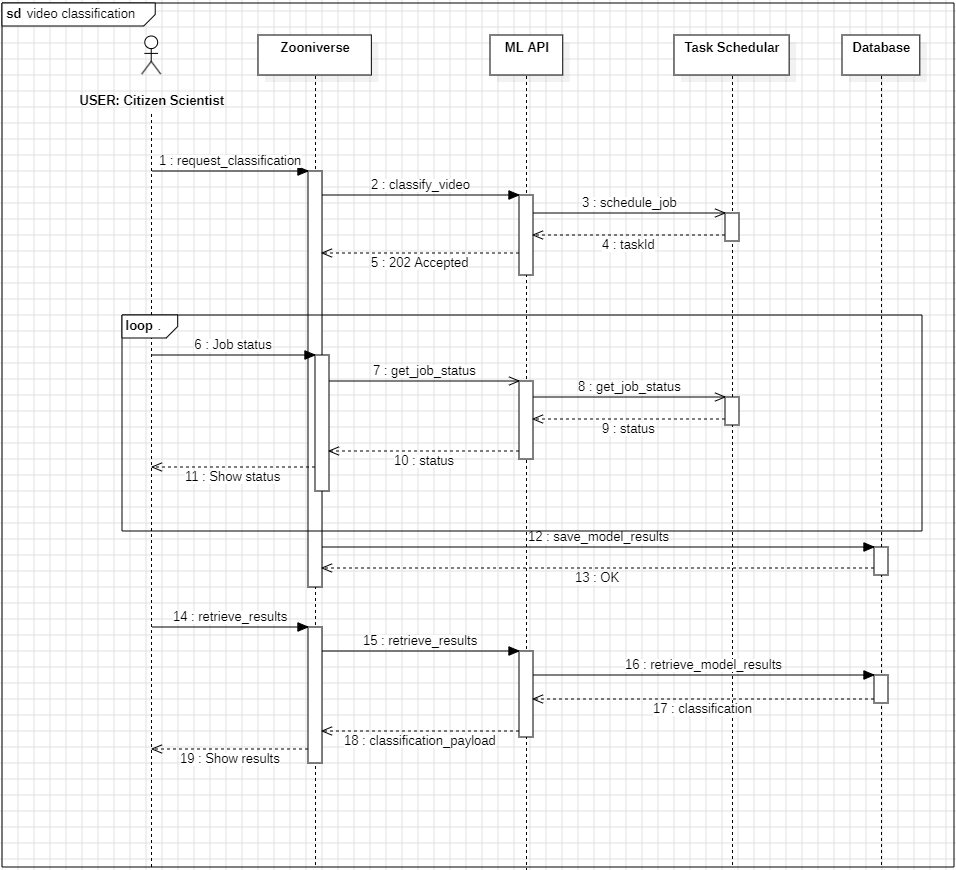
\includegraphics[width=1 \textwidth]{Figures/ImpSequenceDiagram.png}
    \caption{Suggested Sequence Diagram for Video Classification\label{Fig:Improved Sequence Diagram}}
\end{figure}
\subsection{External Interfaces}

\begin{figure}[H]
    \centering
    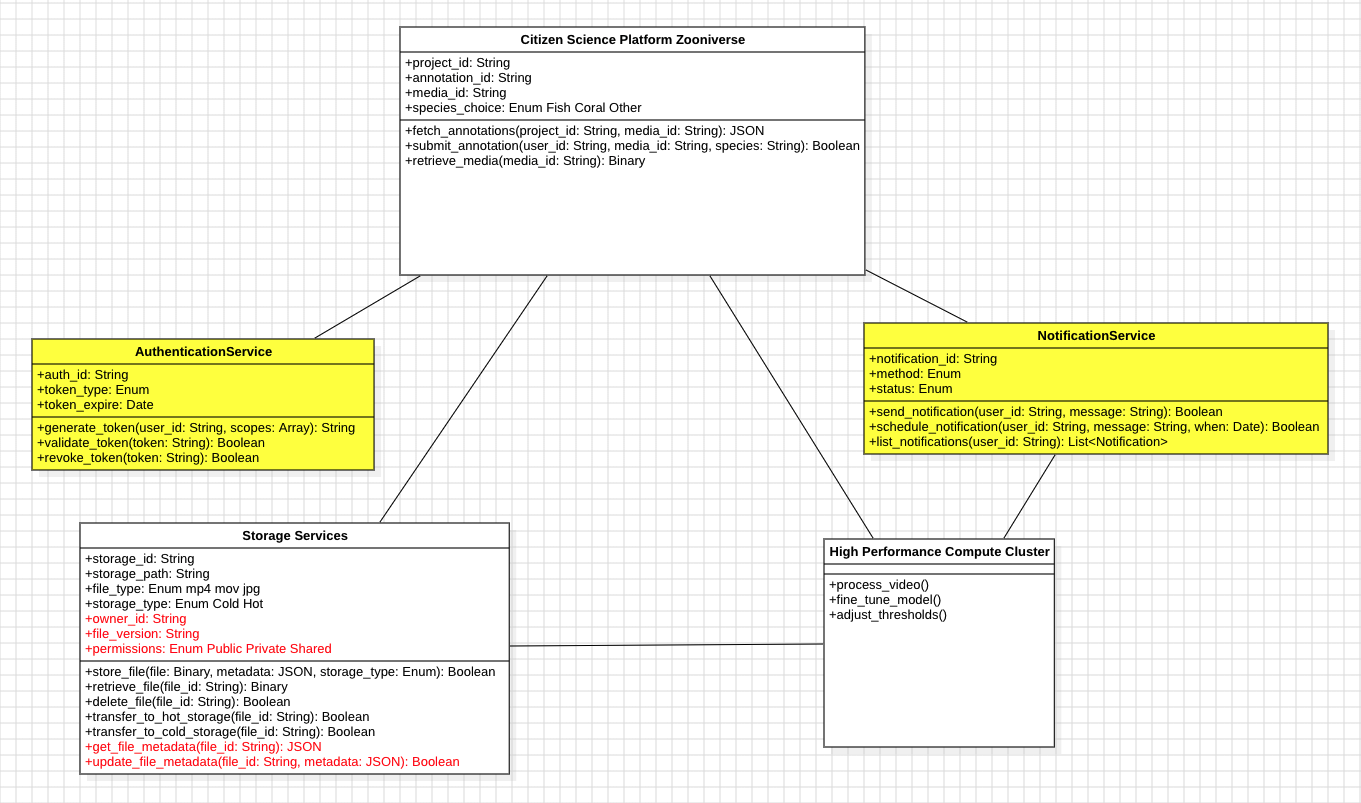
\includegraphics[width=1 \textwidth]{Figures/ImpExternalInterface.png}
    \caption{Improved External Interfaces Class Diagram \label{Fig:Improved External Interfaces Class Diagram}}
\end{figure}
Figure \ref{Fig:Improved External Interfaces Class Diagram} shows our suggestions, let's clarify each of them:
\paragraph{AuthenticationService Interface:}
This external interface provides secure token issuance and validation for all KSO clients (web UI, API gateways, HPC submissions, etc.). KSO issues a REST POST to the Authentication Service with a JSON payload containing \texttt{userId} and requested \texttt{scopes}, and receives back a JSON response with \texttt{accessToken}, \texttt{tokenType} (e.g.\ “Bearer”), and \texttt{expiresIn}. Subsequent calls to any protected KSO endpoint include this token in the \texttt{Authorization} header. The interface also exposes a validation endpoint where KSO can POST a token and receive a Boolean success flag, and a revocation endpoint which invalidates a token before its expiry. Transport is HTTPS, and the service typically implements OAuth 2.0 or SAML under the hood to ensure tokens cannot be forged or replayed.

\paragraph{NotificationService Interface:}
This external interface enables KSO to push alerts and updates to end users or downstream systems via Email, SMS or Webhook. KSO sends a REST POST with a JSON body containing \texttt{recipientId}, \texttt{method} (Email/SMS/Webhook), \texttt{message}, and an optional \texttt{scheduleAt} timestamp; the service returns a JSON containing \texttt{notificationId} and initial \texttt{status} (“PENDING”). KSO can then GET \texttt{/notifications/ \{notificationId\}} to retrieve status transitions (“SENT”, “FAILED”), or DELETE the endpoint to cancel pending deliveries. The service also supports a bulk‐send endpoint for batch notifications and can call back to a KSO‐provided webhook URL upon final delivery, ensuring reliable, asynchronous alerts for long-running tasks.```

\paragraph{StorageService Improvements:}
StorageServices were also improved to enable metadata access, file versioning, permissions, and user-based file listings. The upgrade enables support for handling higher volumes of data more effectively with fine-grained control over file ownership, visibility, and lifecycle. These features are aligned with cloud storage best practices and are required to offer secure, multi-user environments.

\subsection{Interaction scenarios}
\begin{figure}[H]
    \centering
    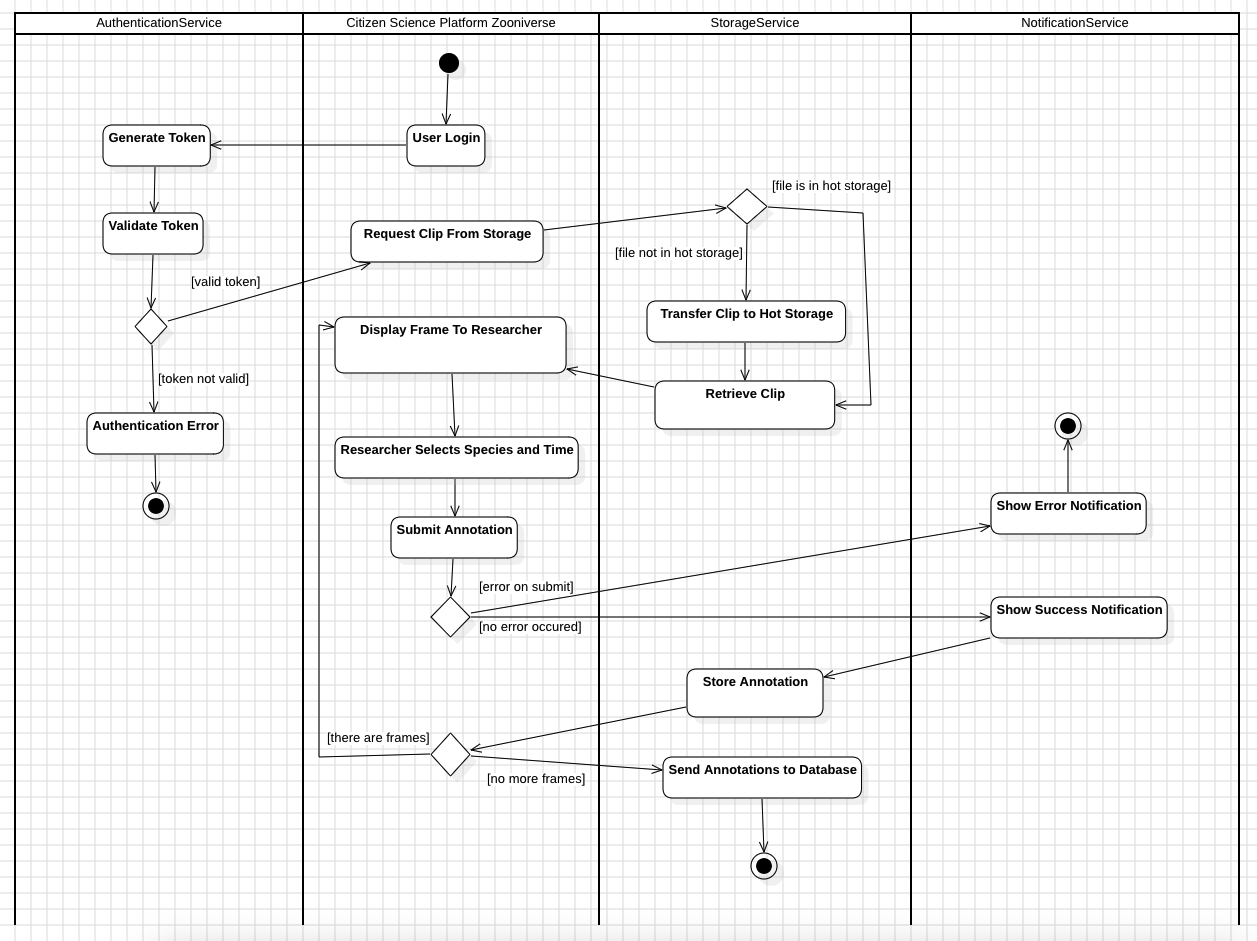
\includegraphics[width=1 \textwidth]{Figures/ImpActivityDiagram.png}
    \caption{Suggested Activity Diagram for Annotate Footage\label{Fig:Improved Activity Diagram}}
\end{figure}

\section{Information View}

\subsection{Stakeholders’ Uses of This View}

The Information View models the structure, attributes, and relationships among the persistent entities of the Koster Seafloor Observatory (KSO) system. With our suggestions, it will capture not only core domain objects but also nuanced metadata and analytical indicators (e.g., bounding boxes, annotation counts, extinction tags). The following stakeholders use this view as follows:

\begin{itemize}
\item \textbf{Database Administrators (DBAs)} – rely on this view to understand both high-level relationships and low-level column details such as \texttt{annotation\_count}, \texttt{bounding\_box}, or \texttt{transfer\_details}. The inclusion of fields like \texttt{metadata\_note} and \texttt{affiliation} helps guide normalization decisions and performance indexing for frequent queries or filtering.
\item \textbf{Backend Developers} – use this diagram to implement data-access layers (e.g., DAOs, repositories). With the new attributes, developers can enrich APIs that support filtering by user \texttt{affiliation}, flag annotations by source (e.g., manual vs. automated), or fetch extinct species data for dynamic UI filtering or validation.
\item \textbf{System Integrators} – benefit from knowing how systems interlink at both object and attribute levels. For example, the ability to link \texttt{ModelAnnotation} to bounding box coordinates and associate it with a specific \texttt{Subject} allows integration with external ML pipelines, which need precise frame-level mapping and model-generated coordinates.
\item \textbf{QA/Test Engineers} – need to verify edge cases such as deletion of a \texttt{Species} that's marked as \texttt{Extinct}, or handling of unexpected \texttt{annotation\_source} values. The \texttt{annotation\_count} field adds another test vector, ensuring consistency between the annotation list and the summary count stored in the \texttt{Subject}.
\item \textbf{Product Owners / Analysts} – gain confidence that new user stories and analytical goals are covered in the schema. The ability to attach \texttt{metadata\_note} to \texttt{Movie} entries, store \texttt{affiliation} per \texttt{User}, or differentiate between annotation origins (human vs. model) supports reporting, traceability, and accountability across the scientific pipeline.
\item \textbf{ML Researchers / Data Scientists} – although not previously listed, this enhanced model now supports their needs. Bounding boxes (\texttt{bounding\_box0}...\texttt{bounding\_box3}), \texttt{confidence}, and \texttt{compareWithAnnotation()} enable direct evaluation of model performance, and the separation of \texttt{annotation\_source} provides a clean way to compare human vs. model accuracy.
\end{itemize}

\subsection{Database Class Diagram}

\begin{figure}[H]
    \centering
    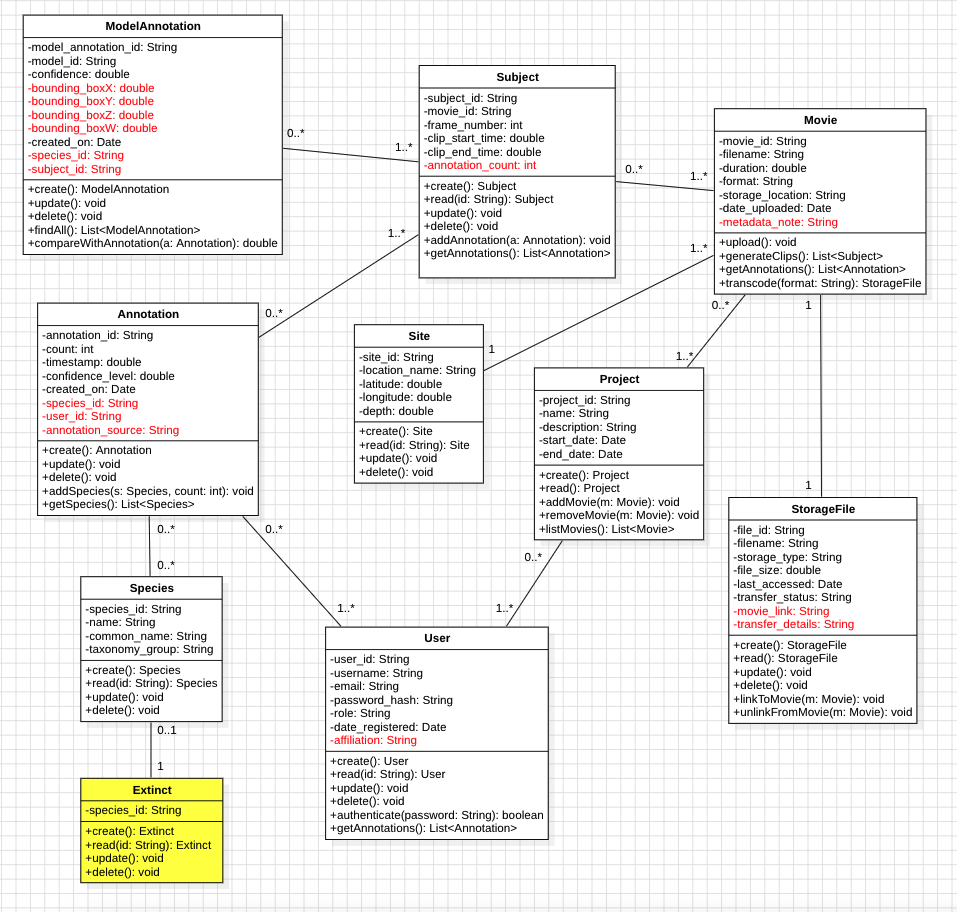
\includegraphics[width=1 \textwidth]{Figures/ImpDatabaseClassDiagram.png}
    \caption{Improved Database Class Diagram \label{Fig:Improved Database Class Diagram}}
\end{figure}

The database class diagram has been extended to support richer domain semantics, improved query performance, and greater analytical depth. These improvements reflect both functional enhancements and new modeling decisions aligned with KSO’s evolving requirements.

\begin{itemize}
\item \textbf{Support for Bounding Boxes and Model Confidence:}
The \texttt{ModelAnnotation} class was extended with bounding box coordinates and a confidence score to enable integration with machine learning pipelines. These additions allow for precise spatial localization of detected features and support downstream evaluation processes, such as comparing model results with human annotations.

\item \textbf{Direct Linking Between Model Outputs and Video Segments:}
A direct reference from \texttt{ModelAnnotation} to \texttt{Subject} was added to allow model predictions to be explicitly associated with individual video clips. This simplifies traceability and improves performance when querying model results for a specific temporal segment.

\item \textbf{Annotation Count Tracking:}
A new attribute in the \texttt{Subject} entity records the total number of linked annotations. This denormalized value supports faster rendering of summary views or dashboards and reduces the need for expensive aggregate queries.

\item \textbf{Metadata Annotations for Movies:}
The \texttt{Movie} class now includes a free-text metadata field that allows users to annotate video files with contextual notes, warnings, or observational remarks. This enriches the interpretability of raw media assets.

\item \textbf{Enhanced File-Movie Association Details:}
The \texttt{StorageFile} class was extended to include both a logical reference to the associated movie and detailed transfer metadata. This supports more transparent storage management and can assist in tracking file provenance or delivery status across systems.

\item \textbf{Annotation Provenance and User Context:}
The \texttt{Annotation} class now captures both the user who submitted the annotation and the origin of the data (e.g., manual vs. automated). This allows system users to differentiate between human-labeled and auto-generated annotations and apply filters accordingly.

\item \textbf{User Affiliation Management:}
An \texttt{affiliation} attribute was added to the \texttt{User} entity to record institutional or organizational context. This is useful for grouping contributors by research group or university, and for generating team-level summaries.

\item \textbf{Extinction Status for Species:}
A new entity was introduced to record species that are extinct. It is linked to \texttt{Species} in a one-to-one relationship and enables special-case handling, such as flagging annotations that reference extinct species or supporting conservation-focused queries.
\end{itemize}

These improvements collectively enhance the schema’s expressiveness, allow for better system performance, and facilitate integration with both scientific workflows and modern analytical tools.


\subsection{Operations on Data}

\begin{longtable}{|l|l|}
\caption{Extended Operations on Data} \label{tab:special-operations} \\
\hline
Operation & Description \\
\hline
\endfirsthead

\multicolumn{2}{c}%
{{\bfseries Table \thetable\ continued from previous page}} \\
\hline
Operation & Description \\
\hline
\endhead

\hline \multicolumn{2}{r}{{Continued on next page}} \\
\endfoot

\hline
\endlastfoot

RecordModelBoundingBox & Create: ModelAnnotation (bounding\_box\_*) \\
                       & Read: ModelAnnotation \\
                       & Update: ModelAnnotation (bounding\_box\_*) \\
                       & Delete: - \\
\hline
LinkModelToSubject & Create: ModelAnnotation (subject\_id) \\
                   & Read: Subject \\
                   & Update: - \\
                   & Delete: - \\
\hline
TrackAnnotationCount & Create: - \\
                     & Read: Subject (annotation\_count) \\
                     & Update: Subject (increment on addAnnotation) \\
                     & Delete: - \\
\hline
AddMovieMetadataNote & Create: - \\
                     & Read: Movie \\
                     & Update: Movie (metadata\_note) \\
                     & Delete: - \\
\hline
LinkMovieInStorage & Create: - \\
                   & Read: StorageFile (movie\_link) \\
                   & Update: StorageFile (movie\_link, transfer\_details) \\
                   & Delete: - \\
\hline
TrackAnnotationSource & Create: Annotation (annotation\_source) \\
                      & Read: Annotation \\
                      & Update: Annotation (source tag change) \\
                      & Delete: - \\
\hline
AttachUserAffiliation & Create: User (affiliation) \\
                      & Read: User \\
                      & Update: User (affiliation) \\
                      & Delete: - \\
\hline
MarkSpeciesAsExtinct & Create: Extinct (species\_id) \\
                     & Read: Species, Extinct \\
                     & Update: Extinct \\
                     & Delete: Extinct \\
\hline
\end{longtable}


\section{Development View}

\subsection{Stakeholders’ Uses of This View}

\begin{itemize}
  \item \textbf{Software Developers} benefit from the addition of the \texttt{LoggingService}, which allows them to emit structured logs during feature development, easing debugging and operational diagnostics. It complements the architectural modularity by offering a standardized logging interface across subsystems.

  \item \textbf{Testers} gain improved visibility into subsystem interactions, as runtime logs can now be analyzed to verify integration correctness and diagnose errors across shared services like the \texttt{MetadataService} and \texttt{TaskScheduler}.

  \item \textbf{System Integrators} use the \texttt{LoggingService} to monitor integration events and validate the operational flow between modules. This ensures smooth orchestration of subsystems such as \texttt{MachineLearningEngine} and \texttt{DataManagement}.

  \item \textbf{Project Managers and Team Leads} are able to use logs generated across subsystems for progress tracking, error trend analysis, and operational health assessments, especially during staging and deployment phases.

  \item \textbf{Maintainers and Evolvers} gain a valuable source of historical and runtime information through logs, which assist in debugging regressions, understanding component behavior, and making informed decisions when evolving the system.

  \item \textbf{Security Engineers} now have access to centralized logs that can be used for forensic analysis, access monitoring, and compliance verification. The presence of a unified logging mechanism simplifies the enforcement of audit policies across the architecture.
\end{itemize}

\subsection{Package Diagram}

\begin{figure}[H]
    \centering
    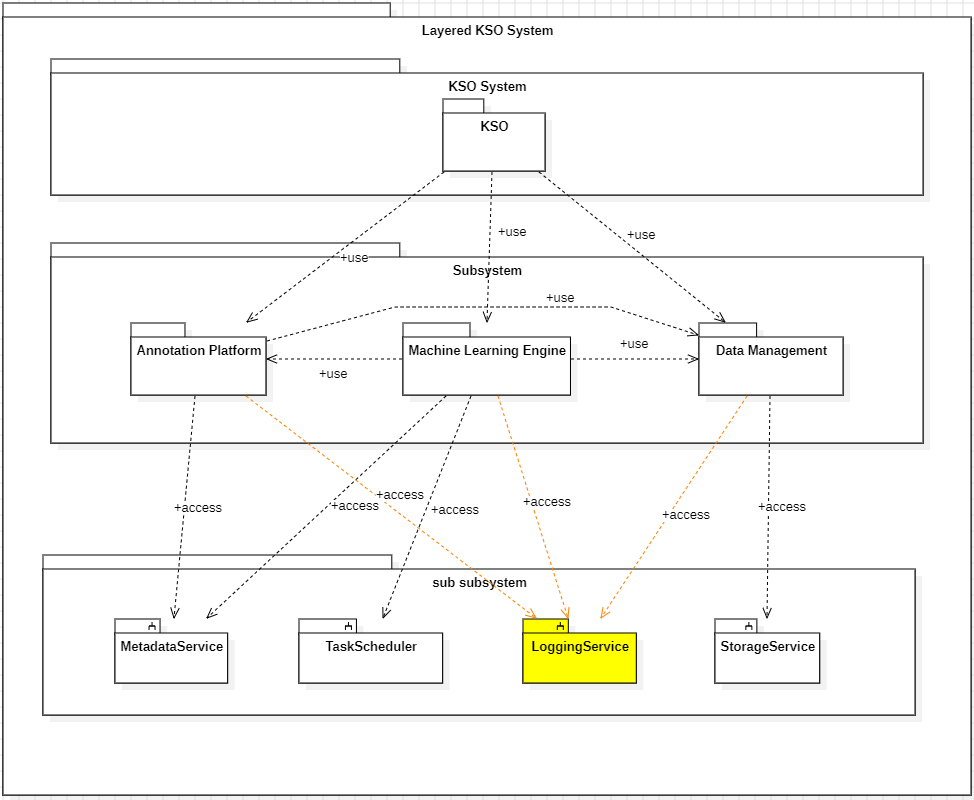
\includegraphics[width=1 \textwidth]{Figures/ImpPackageDiagram.png}
    \caption{Improved Package Diagram \label{Fig:Improved Package Diagram}}
\end{figure}

To improve traceability, observability, and operational transparency across the KSO system, an additional cross-cutting sub-subsystem named \texttt{LoggingService} is introduced at Level 2. This service provides unified logging capabilities to all subsystems, supporting error tracking, audit trails, performance diagnostics, and system monitoring.

At \textbf{Level 2}, the \texttt{LoggingService} becomes a shared technical service accessed by all three Level 1 subsystems. The \texttt{AnnotationPlatform} uses it to record user activities and platform-level exceptions. The \texttt{MachineLearningEngine} logs training progress, inference metrics, and pipeline errors, while \texttt{DataManagement} logs file transfer events, storage health checks, and orchestration outcomes.

This improvement results in the following updated dependencies:
\begin{itemize}
  \item \texttt{AnnotationPlatform} \texttt{→} \texttt{LoggingService}
  \item \texttt{MachineLearningEngine} \texttt{→} \texttt{LoggingService}
  \item \texttt{DataManagement} \texttt{→} \texttt{LoggingService}
\end{itemize}

This change reinforces modularity by isolating operational concerns into a dedicated service and ensures that logs across the system follow a consistent schema, aiding future maintainability and debuggability.

\section{Deployment View}

\subsection{Stakeholders’ Uses of This View}

\begin{itemize}
\item \textbf{System Integrators} 
Use this view to configure connections between the Unified Storage Area, Cloudina Workspace, and HPC Server. They ensure proper mounting and API routing without direct database coupling.

\item \textbf{DevOps and Infrastructure Engineers} 
Plan and manage the deployment of containerized services (e.g., JupyterHub, Metadata API Gateway), storage mounts, and communication protocols such as HTTP, NFS, and SCP.

\item \textbf{Researchers and Data Scientists} 
Leverage the Metadata API to access annotation and species metadata from notebooks, without managing raw SQL or file-based database access. They use shared storage for consistent access to video and training datasets.

\item \textbf{Citizen Science Coordinators} 
Understand the Zooniverse integration path and how annotated data is programmatically fetched, validated, and incorporated into training workflows via the metadata pipeline.

\item \textbf{Marine Biologists and Analysts} 
Gain insight into how field-collected footage (.mp4, .csv) moves from storage to annotation, training, and evaluation, supported by a unified and traceable architecture.
\end{itemize}

\subsection{Deployment Diagram}

\begin{figure}[H]
    \centering
    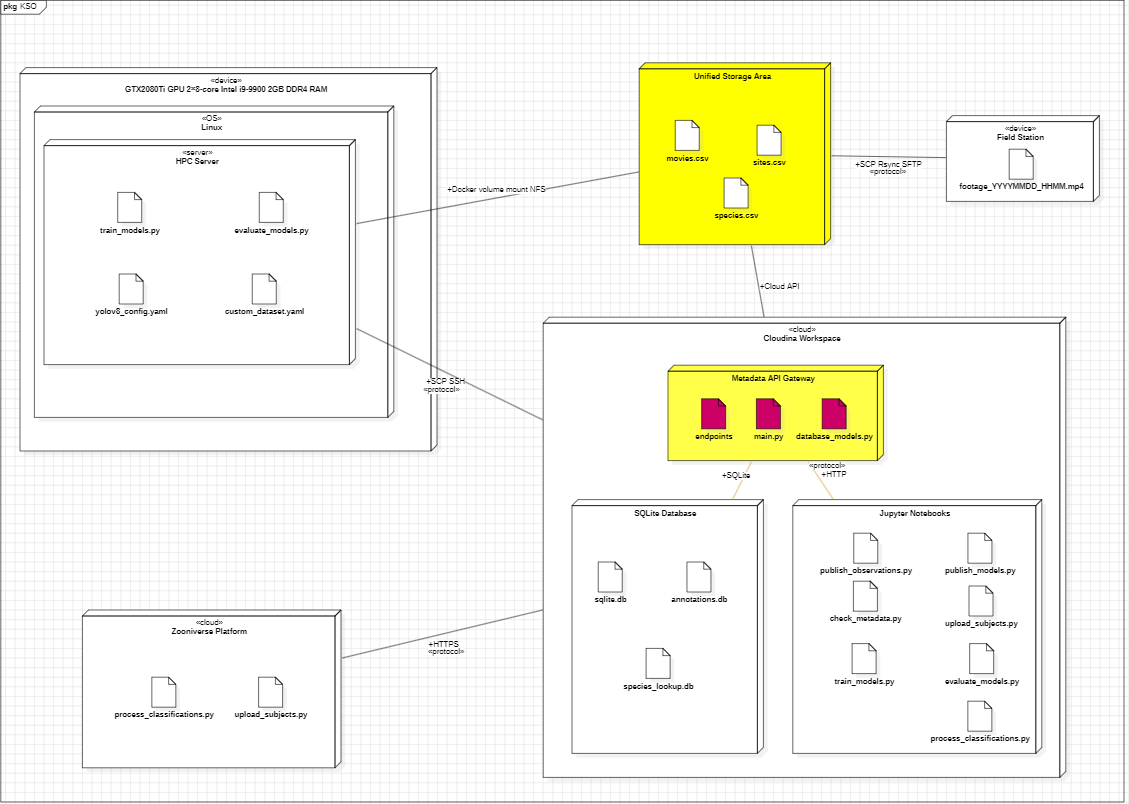
\includegraphics[width=1 \textwidth]{Figures/ImpDeploymentDiagram.png}
    \caption{Improved Deployment Diagram \label{Fig:Improved Deployment Diagram}}
\end{figure}

In the original deployment model, data was separated between Cold Storage (for long-term archival) and Hot Storage (for short-term active use). This introduced unnecessary data duplication, transfer overhead, and potential synchronization issues.

As an improvement, these storage tiers have been merged into a single Unified Storage Area, which retains the semantic distinction between archival and active-use files via directory structure or object tagging (e.g., cold/, hot/, processed/). This storage area is mounted as a shared volume or networked filesystem accessible from both the Cloudina Workspace and the HPC Server, ensuring that; Annotated media, video clips, and derived datasets remain in a consistent, centralized location. Notebooks, training containers, and export processes can access files without manual copying.

Storage management policies (e.g., archival, deletion, versioning) are unified and simplified. This consolidation streamlines operations and enables efficient, reproducible workflows across the system.

In the improved architecture, the Cloudina Workspace no longer accesses the SQLite database directly. Instead, all structured metadata interactions (e.g., querying species, adding annotations, validating sites) are handled through a new internal component: the Metadata API Gateway.

This gateway is deployed within the same environment as the Jupyter notebooks, exposing RESTful endpoints to the notebooks and other internal clients. The API manages all read/write operations to the SQLite database, handling validation, schema abstraction, and request sanitization.

This change brings several benefits; Decouples metadata access from file-based operations, improving security and maintainability. Supports future extensions, such as remote dashboards or data export services, without exposing the raw database. Enforces API contracts, reducing the risk of query mismatches or schema drift.

Together, these improvements form a more modular, reliable, and extensible deployment configuration suitable for scaling citizen science workflows and machine learning pipelines in a production research environment.


\section{Design Rationale}

\begin{itemize}
  \item \textbf{Functional View}: We expanded the core modules by adding \texttt{VideoChunker} and \texttt{AnnotationAggregator} to the Data Management and Citizen Science modules, and \texttt{TrainingOrchestrator} to the Machine Learning module. These components expose new interfaces (\texttt{StorageServices}, \texttt{CitizenSciencePlatform}, \texttt{TaskScheduler}, \texttt{HPCComputeClusterInterface}) that encapsulate video splitting, batch annotation aggregation, and asynchronous training orchestration. This enhances cohesion within each module and decouples workflows, enabling independent evolution and scalable processing.
  \item \textbf{Information View}: We extended the Darwin Core–compliant SQLite schema with new tables—\texttt{Chunks}, \texttt{AnnotationSummaries}, \texttt{JobMetadata}, and \texttt{Logs}—to capture outputs from the VideoChunker, AnnotationAggregator, TrainingOrchestrator, and LoggingService. This maintains standard interoperability for biodiversity data while providing relational support for traceable linkage of video segments, aggregated annotations, training runs, and operational logs.
  \item \textbf{Development View}: The codebase has been refactored into fine-grained packages—\texttt{kso.chunker}, \texttt{kso.annotations}, \texttt{kso.scheduler}, and \texttt{kso.logging}—alongside microservice modules (\texttt{video-chunker-service}, \texttt{annotation-aggregator-service}, \texttt{scheduler-service}, \texttt{logging-service}, \texttt{hpc-gateway}). This modular hierarchy enables parallel workstreams for video, annotation, scheduling, and logging subsystems, reducing merge conflicts and streamlining CI/CD for each service.
  \item \textbf{Deployment View}: Each new component is deployed as a containerized microservice: \texttt{video-chunker} and \texttt{annotation-aggregator} on CPU nodes, \texttt{hpc-gateway} on GPU-enabled HPC nodes, and \texttt{scheduler} and \texttt{logging-service} on dedicated orchestration hosts. The Streamlit front-end and SQLite database remain on general-purpose nodes, while logs are forwarded to an ELK stack. This mapping optimizes resource usage, allows horizontal scaling of batch tasks, and ensures end-to-end observability.
\end{itemize}